
\section{Comparison with simplices}

In \cite[p. 442]{Serre1951homologie}, Serre described a quasi-isomorphism between cubical and simplicial singular chains, also considered in \cite[p.199]{Eilenberg1953acyclic} where is attributed to Cartan.
To describe it let us consider the topological simplex
\begin{equation*}
\gsimplex^n = \{(y_0, \dots, y_n) \mid y_i \in [0,1], \ \textstyle{\sum} \, y_i = 1\}
\end{equation*}
and the topological cube
\begin{equation*}
\gcube^{n} = \{(x_1, \dots, x_n) \mid x_i \in [0,1]\}
\end{equation*}
with their canonical CW structures.
The \textit{Cartan-Serre CW map} $\gcube^n \to \gsimplex^n$ is defined by
\begin{equation} \label{e:cartan-serre CW map}
\begin{split}
&y_0 = 1 - x_1, \\
&y_1 = x_1(1 - x_2), \\
&\ \vdots \\
&y_{n-1} = x_1 x_2 \cdots x_{n-1}(1-x_n), \\
&y_{n} = x_1 x_2 \cdots x_n,
\end{split}
\end{equation}
and is such that, for any space, the induced chain map on singular chain complexes is a quasi-isomorphism.
Furthermore, Serre states that this chain map $S \colon C(\gcube^n) \to C(\gsimplex^n)$ is ``comultiplicative", i.e., it is a coalgebra map where the domain is equipped with the Serre diagonal and the target with the Alexander-Whitney diagonal.

The goal of this section is to prove a generalization of this statement.
We show that $S$ is a morphism of $E_\infty$ coalgebras extending the Serre and Alexander-Whitney diagonals.

We will phrase this statement in the context of cubical and simplicial sets.

The \textit{simplex category} $\simplex$ is the full subcategory of $\Cat$ with objects $[n] = 0 \to 1 \to \cdots \to n$.
Explicitly, its morphisms are generated by the \textit{coface} and \textit{codegeneracy maps} defined by
\begin{align*}
...
\end{align*}

We denote by $\simplex_{\deg}$ the subcategory with the same objects as $\simplex$ and morphisms of the form $\sigma_i \circ \tau$ for some morphisms $\tau$ of $\simplex$.

The category of \textit{simplicial sets} is the functor category $\sSet = \Fun(\simplex^\op, \Set)$.
The \textit{standard $n$-simplex} is the cubical set $\simplex^n = \simplex(-, [n])$, and the \textit{Yoneda embedding} $\simplex \to \sSet$ is the functor induced by $[n] \mapsto \simplex^n$.
For any cubical set $X$ we have
\begin{equation*}
X_n \cong \colim_{\simplex^n \to X} \simplex^n.
\end{equation*}

The functor of \textit{(normalized) chains} $\cchains \colon \sSet \to \Ch$ is the Kan extension along the Yoneda embedding of the functor $\simplex \to \Ch$ assigning to $[n]$ in degree $m$ the $R-module$
\begin{equation*}
\frac{R\{\simplex([m], [n])\}}{R\{\simplex_{\deg}([m], [n])\}}
\end{equation*}
and whose boundary is defined by
\begin{equation*}
\partial (\id_{[n]}) = \sum_{i=0}^{n} (-1)^i \ \id_{[n]} \circ \delta_i.
\end{equation*}
We remark that $\chains(\simplex^n)$ is isomorphic to the cellular chains on $\gsimplex^n$, whose faces are parameterized by ordered tuples of vertices $[v_0, \dots, v_m]$.

In \cite{Medina20prop1}, a similar construction to the one introduced in Section~\ref{s:coaction} provides the chains of simplicial sets with a natural $U(\M)$-coalgebra structure.
It is also induced from a natural $\M$-bialgebra structure on the chains of standard simplices.
This $\M$-bialgebra structure on $\chains(\simplex^n)$ is defined by the assignment
\begin{equation*}
\counit \mapsto \epsilon, \quad \coproduct \mapsto \Delta, \quad \product \mapsto \ast,
\end{equation*}
where
\begin{equation*}
\varepsilon \big( [v_0, \dots, v_q] \big) = \begin{cases} 1 & \text{ if } q = 0, \\ 0 & \text{ if } q > 0, \end{cases}
\end{equation*}
is the \textit{augmentation map},
\begin{equation*}
\Delta \big( [v_0, \dots, v_q] \big) = \sum_{i=0}^q [v_0, \dots, v_i] \otimes [v_i, \dots, v_q],
\end{equation*}
is the \textit{Alexander-Whitney diagonal}, and
\begin{equation*}
\left[v_0, \dots, v_p \right] \ast \left[v_{p+1}, \dots, v_q\right] = \begin{cases} (-1)^{p+|\pi|} \left[v_{\pi(0)}, \dots, v_{\pi(q)}\right] & \text{ if } v_i \neq v_j \text{ for } i \neq j, \\
0 & \text{ if not}, \end{cases}
\end{equation*}
where $\pi$ is the permutation that orders the totally ordered set of vertices and $(-1)^{|\pi|}$ is its sign, is an algebraic version of the \textit{join}.

We use a triple $(F_0, F_{01}, F_1)$ of sets to represent a face $F$ of $\gcube^n$, requiring that they form a partition of $\{1, \dots, n\}$ and for $\epsilon \in \{0,1\}$, $F_\epsilon = \{i \mid \forall x \in F, \, x_i = \epsilon\}$. 
Given a subset $U = \{u_1 < \cdots < u_q\}$ of $\{0, \dots, n\}$ we write $d_U$ for $d_{u_1} \! \cdots \, d_{u_q}$.
In this notation, any face of $\simplex^n$ can be written as $d_U [0, \dots, n]$ for some $U$.

With this notation we have the following description of the Cartan-Serre chain map.

\begin{lemma}
	On basis elements $S \colon \cchains(\cube^n) \to \chains(\triangle^n)$ is given by
	\begin{equation*}
	(F_0, F_{0,1}, F_1) \mapsto
	\begin{cases}
	d_U [0, \dots, n] & \text{ if } F_{01} \cap \{i \mid i > \min(F_0)\} = \emptyset, \\
	0 & \text{ otherwise},
	\end{cases}
	\end{equation*}
	where $U = \{i-1 \mid i \in F_1 \text{ or } i > \min(F_0)\}$ with the convention $\min \emptyset = +\infty$.
\end{lemma}

\begin{proof}
	We assume $n > 0$ since otherwise there is nothing to prove.
	Consider a face $(F_0, F_{01}, F_1)$ and let $M \subseteq \{0, \dots, n\}$ be empty if $F_0$ is empty or be characterized by $i > \min (F_0)$ otherwise.
	Notice in \eqref{e:cartan-serre CW map} that if $x_i = 0$ then $y_j = 0$ for every $j > i$.
	Therefore, the image of $(F_0, F_{01}, F_1)$ in $\simplex^n$ is a face of $d_U[0, \dots, n]$ where $U = \{i-1 \mid i \in M\}$ or, more explicitly, $[0, \dots, n]$ if $F_0$ is empty and $[0, \dots, \min(F_0)]$ otherwise.
	In particular, $S(F_0, F_{01}, F_1)$ is non-zero only if $M \cap F_{01} = \emptyset$, and we can assume without loss of generality that $F_0 = \emptyset$ or $F_0 = \{n\}$.

	Notice from \eqref{e:cartan-serre CW map} that $x_i = 1$ if and only if $y_{i-1} = 0$, so $S(\emptyset, F_{01}, F_1) = d_{U} [0, \dots, n]$ where $U = \{i-1 \mid i \in F_1\}$.
\end{proof}


This chain map is not in general a morphism of $\M$-bialgebras, for example, notice that $S([0] \otimes [0,1]) = 0$, but $([1] \otimes [1]) \ast ([0] \otimes [0,1]) = -([0,1] \otimes [0,1])$ which is mapped to $-[0,1,2]$ by $S$.

To make $S$ into an $E_\infty$ coalgebra map we restrict the $\M$-bialgebra structures on $C(\gcube^n)$ and $C(\simplex^n)$ to an $E_\infty$ suboperad of $U(\M)$ which we now describe.

We will utilize the following diagrammatic simplification
\begin{center}
	\boxed{\begin{tikzpicture}[scale=.4]
		\draw (6,2)--(7,1)--(7,0);
		\draw (8,2)--(7,1);
		\node at (6,2.5){$\scriptstyle 1$};
		\node at (7,2.5){$\scriptstyle \dots$};
		\node at (8,2.5){$\scriptstyle n$};
		
		\draw (11,.5)--(12,1.5)--(12,2.5);
		\draw (13,.5)--(12,1.5);
		\node at (11,0){$\scriptstyle 1$};
		\node at (12,0){$\scriptstyle \dots$};
		\node at (13,0){$\scriptstyle n$};
		\end{tikzpicture}}
\end{center}
to represent labeled directed graphs resulting from iterated grafting of \product and \coproduct \ in the left comb order
\begin{center}
	\boxed{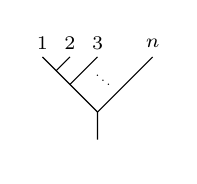
\begin{tikzpicture}[scale=.35]		
		\node at (-2.15,-.25){};
		\node at (-2.15,3.25){};
		
		\node at (-2,3.5){$\scriptstyle 1$};
		\node at (-1,3.5){$\scriptstyle 2$};
		\node at (0,3.5){$\scriptstyle 3$};
		\node at (2,3.5){$\scriptstyle n$};
		
		\draw (-2,3)--(0,1);
		\draw (2,3)--(0,1)--(0,0);
		\draw (0,3)--(-1,2);
		\draw (-1,3)--(-1.5,2.5);
		\draw (.2,2.3) node[scale= 0.5] {$\ddots$};
		\end{tikzpicture}
		\qquad 
		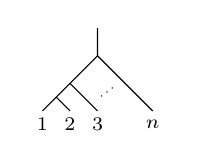
\begin{tikzpicture}[scale=.35]	
		
		\node at (-2,-3.5){$\scriptstyle 1$};
		\node at (-1,-3.5){$\scriptstyle 2$};
		\node at (0,-3.5){$\scriptstyle 3$};
		\node at (2,-3.5){$\scriptstyle n$};
		
		\draw (-2,-3)--(0,-1);
		\draw (2,-3)--(0,-1)--(0,0);
		\draw (0,-3)--(-1,-2);
		\draw (-1,-3)--(-1.5,-2.5);
		\draw (.2,-2.3) node[scale= 0.5, rotate = 75] {$\ddots$};
		\end{tikzpicture}}
\end{center}

A \textit{surjection-like graph} is either the $(1,0)$-graph \counit\ or for $n > 1$ a $(1, n)$-graph of the form 
\begin{center}
\boxed{\begin{tikzpicture}[scale=.4]
	\node at (5,8){$\scriptstyle 1$};
	\draw (3,5.5)--(5,6.5)--(5,7.5);
	\draw (7,5.5)--(5,6.5);
	\node at (3,5){$\scriptstyle 1$};
	\node at (5,5){\,$\scriptstyle \dots$};
	\node at (7,5){$\scriptstyle r+d$};
	
	\node at (5,4){$\vdots$};
	
	\node at (3,-.5){$\scriptstyle 1$};
	\draw (2,2)--(3,1)--(3,0);
	\draw (4,2)--(3,1);
	\node at (2,2.5){$\scriptstyle 1$};
	\node at (3,2.5){$\scriptstyle \dots$};
	\node at (4,2.5){$\scriptstyle k_1$};
	
	\node at (5,1){\ $\cdots$};
	
	\node at (7,-.5){$\scriptstyle r$};
	\draw (6,2)--(7,1)--(7,0);
	\draw (8,2)--(7,1);
	\node at (6,2.5){$\scriptstyle 1$};
	\node at (7,2.5){$\scriptstyle \dots$};
	\node at (8,2.5){$\scriptstyle k_r$};
	\end{tikzpicture}}
\end{center}
containing no internal vertices and such that for each $i = 1, \dots, r$ the induced map 
\begin{equation*}
\{1, \dots, k_i\} \to \{1, \dots, r+d\}
\end{equation*}
is order preserving.

Let $\MS$ be the sub-prop of $\M$ generated by elements represented by surjection-like graphs.
The associated operad $U(\MS)$ was used in \cite[Theorem A.11.]{Medina20prop1} to compare the action of the surjection operad of McClure-Smith \cite{McClure} and Berger-Fresse \cite{Berger} on simplicial sets and that of $U(\M)$.
The same proof used in \cite[Theorem 3.3.]{Medina20prop1} shows $U(\MS)$ is an $E_\infty$ operad.
The proof of the following result occupies Section~\ref{s:proof2}.
 
\begin{theorem} \label{t:comparison}
	Let $X$ be a cubical set and $Y$ a simplicial set.
	The Cartan-Serre chain map $S \colon \cchains(X) \to \chains(Y)$ is a morphism of $U(\MS)$-coalgebras.
\end{theorem}